\chapter{Droites et systèmes}

\section{Systèmes d'équations à 2 inconnues}

\begin{df}
	Soit $a$, $b$, $c$, $a'$, $b'$ et $c'$ des nombres réels donnés.

	On appelle \textbf{système de deux équations linéaires à deux inconnues} $x$ et $y$ une expression de la forme :
	\[
		(S):\begin{cases}
			ax + by = c \\
			a'x + b'y = c'
		\end{cases}
	\]

	Un couple de réels $\coordl{x}{y}$ qui vérifie simultanément les deux équations est appelé \textbf{solution} du système.
\end{df}

\begin{ex}
	On considère le système :
	\[
		(S):\begin{cases}
			2x - y = 0 \\
			3x - 4y = -5
		\end{cases}
	\]

	Le couple $\coordl{1}{2}$ est solution du système car :
	\[
		\begin{cases}
			2 \times 1 - 2 = 0 \\
			3 \times 1 - 4 \times 2 = -5
		\end{cases}
	\]
\end{ex}

\subsection{Méthode de substitution}

\begin{methode}[Résoudre un système par substitution]
	Cette méthode consiste à exprimer une inconnue en fonction de l'autre à partir d'une des deux équations, puis à la substituer dans la seconde équation.

	On privilégie cette méthode lorsqu'une inconnue a un coefficient égal à $1$ ou $-1$.
\end{methode}

\begin{ex}
	Résoudre le système :
	\[
		(S_1):\begin{cases}
			3x + 2y = 0 \\
			x - 4y = 14
		\end{cases}
	\]

	\begin{correction}
		\nline
		\begin{align*}
			(S_1):\begin{cases} 3x + 2y = 0 \\ x - 4y = 14 \end{cases} & \iff \begin{cases} 3x + 2y = 0 \\ \boxed{x = 14 + 4y} \end{cases} \quad \text{\small (On isole $x$ dans la $2^\text{e}$ équation)}                                                   \\
			                                                           & \iff \begin{cases} 3\times\boxed{(14 + 4y)} + 2y = 0 \\ x = 14 + 4y \end{cases} \quad \text{\small (On substitue $x$ dans la $1^\text{re}$ équation)}                                \\
			                                                           & \iff \begin{cases} 42 + 12y + 2y = 0 \\ x = 14 + 4y \end{cases} \iff \begin{cases} 14y = -42 \\ x = 14 + 4y \end{cases} \iff \begin{cases} \boxed{y = -3} \\ x = 14 + 4y \end{cases} \\
			                                                           & \iff
			\begin{cases}
				\boxed{y = -3}                 &                                                                        \\
				x = 14 + 4 \times \boxed{(-3)} & \text{\small (On remplace $y$ par $-3$ dans la $2^\text{e}$ équation)}
			\end{cases}
			\iff
			\begin{cases} y = -3 \\ x = 2 \end{cases}
		\end{align*}

		La solution du système est le couple $\coordl{2}{-3}$. On note : $S = \{\coordl{2}{-3}\}$.
	\end{correction}
\end{ex}

\subsection{Méthode des combinaisons linéaires}

\begin{methode}[Résoudre un système par combinaisons linéaires]
	Cette méthode consiste à multiplier les équations par des coefficients adéquats afin d'obtenir des coefficients identiques ou opposés pour l'une des inconnues, puis à additionner ou soustraire membre à membre les équations pour éliminer cette inconnue.
\end{methode}

\begin{ex}
	Résoudre les systèmes suivants :

	\begin{multicols}{2}
		\begin{itemize}
			\item $(S_1):\begin{cases} 3x - 2y = 11 \\ 6x + 3y = 15 \end{cases}$
			\item $(S_2):\begin{cases} 3x - 2y = 7 \\ 5x + 3y = -1 \end{cases}$
		\end{itemize}
	\end{multicols}

	\begin{correction}
		\nline
		\begin{itemize}
			\item Pour résoudre $(S_1)$ :
			      \begin{itemize}
				      \item On multiplie la $1^\text{re}$ équation par $2$ pour égaliser les coefficients de $x$ :
				            \[
					            (S_1):\begin{cases}
						            3x - 2y = 11 & (\times 2) \\
						            6x + 3y = 15
					            \end{cases}
					            \iff
					            \begin{cases}
						            6x - 4y = 22 \\
						            6x + 3y = 15
					            \end{cases}
				            \]

				      \item On soustrait la $2^\text{e}$ équation de la $1^\text{re}$ pour éliminer $x$ :
				            \[
					            \begin{array}{rrcl}
						                 & (6x - 4y) - (6x + 3y) & = & 22 - 15 \\
						            \iff & -7y                   & = & 7       \\
						            \iff & y                     & = & -1
					            \end{array}
				            \]

				      \item On remplace $y = -1$ dans la première équation $3x - 2y = 11$ :
				            \[
					            \begin{array}{rrcl}
						                 & 3x - 2 \times (-1) & = & 11               \\
						            \iff & 3x + 2             & = & 11               \\
						            \iff & 3x                 & = & 9 \implies x = 3
					            \end{array}
				            \]

				            La solution du système est le couple $\coordl{3}{-1}$. On note : $S = \{\coordl{3}{-1}\}$.
			      \end{itemize}

			\item Pour résoudre $(S_2)$ :
			      \begin{itemize}
				      \item On multiplie la $1^\text{re}$ par $5$ et la $2^\text{e}$ par $3$ pour obtenir le même coefficient devant $x$ :
				            \[
					            (S_2):\begin{cases}
						            3x - 2y = 7  & (\times 5) \\
						            5x + 3y = -1 & (\times 3)
					            \end{cases}
					            \iff
					            \begin{cases}
						            15x - 10y = 35 \\
						            15x + 9y = -3
					            \end{cases}
				            \]

				      \item On soustrait les deux équations :
				            \[
					            \begin{array}{rrcl}
						                 & (15x - 10y) - (15x + 9y) & = & 35 - (-3) \\
						            \iff & -19y                     & = & 38        \\
						            \iff & y                        & = & -2
					            \end{array}
				            \]

				      \item On remplace $y = -2$ dans $3x - 2y = 7$ :
				            \begin{align*}
					            3x - 2 \times (-2) & = 7                \\
					            3x + 4             & = 7                \\
					            3x                 & = 3 \implies x = 1
				            \end{align*}

				            La solution du système est le couple $\coordl{1}{-2}$. On note : $S = \{\coordl{1}{-2}\}$.
			      \end{itemize}
		\end{itemize}
	\end{correction}
\end{ex}


\section{Résolutions et interprétations graphiques}

Soit $a, b, c, a', b', c'$ des réels avec $b \neq 0$ et $b' \neq 0$.

Le système $(S) : \begin{cases} ax + by = c \\ a'x + b'y = c' \end{cases}$ équivaut à la donnée des deux équations réduites de droites :
\[
	(d) : y = -\frac{a}{b}x + \frac{c}{b}
	\qquad \text{et} \qquad
	(d') : y = -\frac{a'}{b'}x + \frac{c'}{b'}
\]

La résolution du système correspond à l'étude de la position relative des droites $(d)$ et $(d')$.

\begin{propriete}[Interprétation graphique d'un système d'équations]
	Soit $(S)$ le système $\begin{cases} ax + by = c \\ a'x + b'y = c' \end{cases}$.
	\begin{itemize}
		\item \textbf{Unique solution :} Le système $(S)$ admet un unique couple solution si et seulement si les droites $(d)$ et $(d')$ sont sécantes, c'est-à-dire si leurs coefficients directeurs sont différents :
		      \[
			      -\frac{a}{b} \neq -\frac{a'}{b'} \iff ab' \neq a'b \iff ab' - a'b \neq 0
		      \]

		      Le couple solution est alors formé par les coordonnées du point d'intersection des deux droites.
		\item \textbf{Aucune solution :} Si $ab' - a'b = 0$ (coefficients directeurs égaux) et $\dfrac{c}{b}\neq\dfrac{c'}{b'}$, les droites $(d)$ et $(d')$ sont strictement parallèles.

		      Le système n'admet aucune solution. On note $S = \emptyset$.
		\item \textbf{Une infinité de solutions :} Si $ab' - a'b = 0$ (coefficients directeurs égaux) et $\dfrac{c}{b}=\dfrac{c'}{b'}$, les droites $(d)$ et $(d')$ sont confondues.

		      Le système admet une infinité de solutions qui sont tous les couples $\coordl{x}{y}$ correspondant aux coordonnées des points de cette droite. On note : $S=\brac{\coordl{x}{y}\quad\text{tel que}\quad ax+by=c}$
	\end{itemize}
	\begin{center}
		\begin{tikzpicture}[scale=0.7, >=Stealth]
			\begin{scope}[shift={(0,0)}]
				\draw[step=0.5cm, gray!20, very thin] (-1.8,-1.8) grid (2.8,2.8);
				\draw[->, thick] (-1.8,0) -- (2.8,0) node[right] {\small $x$};
				\draw[->, thick] (0,-1.8) -- (0,2.8) node[above] {\small $y$};
				\draw[domain=-1.5:2.5, smooth, variable=\x, blue, thick] plot (\x, {0.8*\x + 0.2}) node[above] {\small $(d)$};
				\draw[domain=-0.8:2.5, smooth, variable=\x, red, thick] plot (\x, {-1.2*\x + 2.2}) node[right] {\small $(d')$};
				\filldraw[black] (1,1) circle (2pt);
				\draw[dashed, thin] (1,0) node[below] {\small $x_0$} -- (1,1) -- (0,1) node[left] {\small $y_0$};
				\node[align=center, below] at (0.5,-2.2) {\small \textbf{Droites sécantes}\\[-0.2em]\footnotesize Unique solution};
			\end{scope}
			\begin{scope}[shift={(8,0)}]
				\draw[step=0.5cm, gray!20, very thin] (-1.8,-1.8) grid (2.8,2.8);
				\draw[->, thick] (-1.8,0) -- (2.8,0) node[right] {\small $x$};
				\draw[->, thick] (0,-1.8) -- (0,2.8) node[above] {\small $y$};
				\draw[domain=-1.8:2.2, smooth, variable=\x, blue, thick] plot (\x, {0.7*\x + 1}) node[above] {\small $(d)$};
				\draw[domain=-1.2:2.8, smooth, variable=\x, red, thick] plot (\x, {0.7*\x - 0.8}) node[right] {\small $(d')$};
				\node[align=center, below] at (0.5,-2.2) {\small \textbf{Droites parallèles}\\[-0.2em]\footnotesize Aucune solution};
			\end{scope}
			\begin{scope}[shift={(16,0)}]
				\draw[step=0.5cm, gray!20, very thin] (-1.8,-1.8) grid (2.8,2.8);
				\draw[->, thick] (-1.8,0) -- (2.8,0) node[right] {\small $x$};
				\draw[->, thick] (0,-1.8) -- (0,2.8) node[above] {\small $y$};
				\draw[domain=-1.5:2.5, smooth, variable=\x, blue, thick] plot (\x, {-0.6*\x + 0.8});
				\draw[domain=-1.5:2.5, smooth, variable=\x, red, dashed, ultra thick] plot (\x, {-0.6*\x + 0.8});
				\node[purple,anchor=west] at (2.5,-0.6) {\small $(d) = (d')$};
				\node[align=center, below] at (0.5,-2.2) {\small \textbf{Droites confondues}\\[-0.2em]\footnotesize Infinité de solutions};
			\end{scope}
		\end{tikzpicture}
	\end{center}
\end{propriete}

\begin{methode}[Système admettant une unique solution]
	Résoudre graphiquement le système :
	\[
		(S):\begin{cases}
			-2x + y = 0 \\
			4x - y = 4
		\end{cases}
	\]

	\begin{correction}
		On met chaque équation sous forme réduite $y = \dots$ :
		\[
			(S):\begin{cases} -2x + y = 0 \\ 4x - y = 4 \end{cases} \iff \begin{cases} y = 2x \\ y = 4x - 4 \end{cases}
		\]

		On trace dans un repère les deux droites d'équations $y = 2x$ et $y = 4x - 4$.

		\begin{center}
			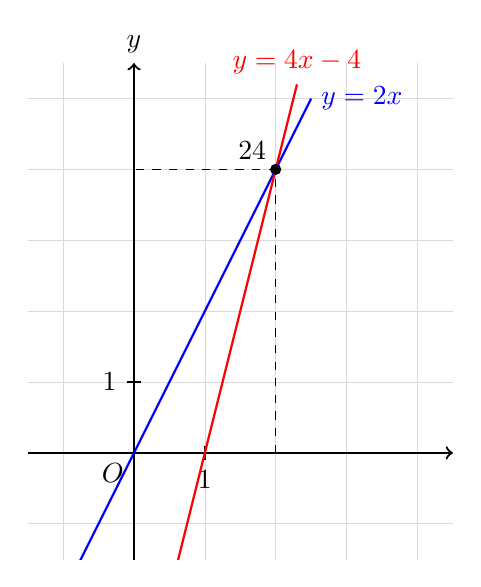
\begin{tikzpicture}[scale=0.9]
				\clip (-1.5,-1.5) rectangle (4.5,6);
				\draw[step=1cm, gray!30, very thin] (-1.5,-4.5) grid (4.5,5.5);
				\draw[->, thick] (-1.5,0) -- (4.5,0) node[right] {$x$};
				\draw[->, thick] (0,-4.5) -- (0,5.5) node[above] {$y$};
				\draw[thick] (0,0) node[below left] {$O$};
				\draw[thick] (1,0.1) -- (1,-0.1) node[below] {$1$};
				\draw[thick] (0.1,1) -- (-0.1,1) node[left] {$1$};
				\draw[domain=-1.5:2.5, smooth, variable=\x, blue, thick] plot (\x, {2*\x}) node[right] {$y=2x$};
				\draw[domain=-0.1:2.3, smooth, variable=\x, red, thick] plot (\x, {4*\x - 4}) node[above] {$y=4x-4$};
				\filldraw[black] (2,4) circle (2pt) node[above left] {$\coordl{2}{4}$};
				\draw[dashed] (2,0) -- (2,4) -- (0,4);
			\end{tikzpicture}
		\end{center}

		Les solutions sont les coordonnées du point d'intersection des deux droites.

		Par lecture graphique, la solution est le couple $\coordl{2}{4}$.

		On note : $S = \{\coordl{2}{4}\}$.
	\end{correction}
\end{methode}

\begin{methode}[Système sans solution]
	Démontrer que le système suivant n'admet pas de solution :
	\[
		(S):\begin{cases}
			-3x + y = 1 \\
			6x - 2y = 6
		\end{cases}
	\]

	\begin{correction}
		On met chaque équation sous forme réduite :
		\[
			(S):\begin{cases} -3x + y = 1 \\ 6x - 2y = 6 \end{cases} \iff \begin{cases} y = 3x + 1 \\ -2y = -6x + 6 \end{cases} \iff \begin{cases} y = 3x + 1 \\ y = 3x - 3 \end{cases}
		\]

		Les deux droites ont :
		\begin{itemize}
			\item Le même coefficient directeur $3$
			\item Des ordonnées à l'origine différents car $(+1)\neq(-3)$
		\end{itemize}

		Elles sont strictement parallèles et n'ont aucun point d'intersection, donc $\pa{S}$ n'admet pas de solution.

		On note : $S = \emptyset$.

		\begin{center}
			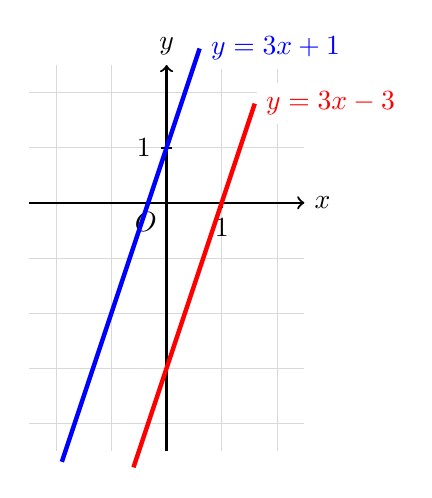
\begin{tikzpicture}[scale=0.7]
				\draw[step=1cm, gray!30, very thin] (-2.5,-4.5) grid (2.5,2.5);
				\draw[->, thick] (-2.5,0) -- (2.5,0) node[right] {$x$};
				\draw[->, thick] (0,-4.5) -- (0,2.5) node[above] {$y$};
				\node[below left] at (0,0) {$O$};
				\draw[thick] (1,0.1) -- (1,-0.1) node[below] {$1$};
				\draw[thick] (0.1,1) -- (-0.1,1) node[left] {$1$};
				\draw[domain=-1.9:0.6, smooth, variable=\x, blue, ultra thick] plot (\x, {3*\x + 1}) node[right, fill=white] {$y=3x+1$};
				\draw[domain=-0.6:1.6, smooth, variable=\x, red, ultra thick] plot (\x, {3*\x - 3}) node[right, fill=white] {$y=3x-3$};
			\end{tikzpicture}
		\end{center}
	\end{correction}
\end{methode}

\begin{methode}[Système avec une infinité de solutions]
	Démontrer que le système suivant admet une infinité de solutions :
	\[
		\begin{cases}
			-6x - 3y = -6 \\
			2x + y = 2
		\end{cases}
	\]

	\begin{correction}
		On met chaque équation sous forme réduite :
		\[
			\begin{cases}
				-6x - 3y = -6 \\
				2x + y = 2
			\end{cases}
			\iff
			\begin{cases}
				-3y = 6x - 6 \\
				y = -2x + 2
			\end{cases}
			\iff
			\begin{cases}
				y = -2x + 2 \\
				y = -2x + 2
			\end{cases}
		\]

		Les deux droites ont la même équation réduite donc elles sont confondues et possèdent une infinité de points d'intersection.

		Le système admet donc une infinité de solutions : tous les couples $\coordl{x}{y}$ vérifiant $y = -2x + 2$.

		On note : $S = \brac{\coordl{x}{y}\quad\text{tel que}\quad y = -2x + 2}$.
	\end{correction}
	\begin{center}
		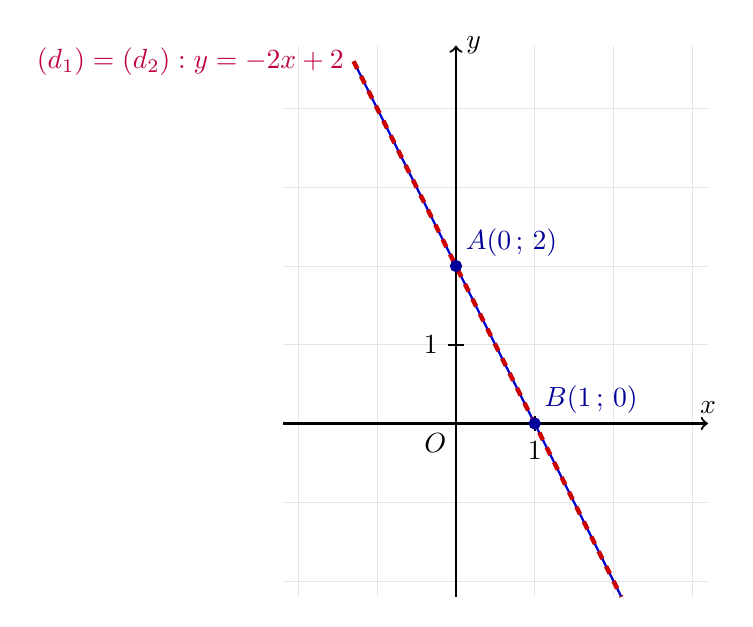
\begin{tikzpicture}
			\draw[step=1cm, gray!20, very thin] (-2.2,-2.2) grid (3.2,4.8);
			\draw[->, thick] (-2.2,0) -- (3.2,0) node[above] {$x$};
			\draw[->, thick] (0,-2.2) -- (0,4.8) node[right] {$y$};
			\node[below left] at (0,0) {$O$};
			\draw[thick] (1,0.1) -- (1,-0.1) node[below] {$1$};
			\draw[thick] (0.1,1) -- (-0.1,1) node[left] {$1$};
			\draw[domain=-1.3:2.1, smooth, variable=\x, blue!80!black, thick] plot (\x, {-2*\x + 2});
			\draw[domain=-1.3:2.1, smooth, variable=\x, red!80!black, ultra thick, dashed] plot (\x, {-2*\x + 2});
			\filldraw[blue!60!black] (0,2) circle (2pt) node[above right] {$A(0\,;\,2)$};
			\filldraw[blue!60!black] (1,0) circle (2pt) node[above right] {$B(1\,;\,0)$};
			\node[purple, anchor=east] at (-1.3, 4.6) {$(d_1) = (d_2) : y = -2x + 2$};
		\end{tikzpicture}
	\end{center}
\end{methode}
